\chapter{Transformer Networks}
\label{ch-transformer}

The primary reference for this chapter is  Ref.\cite{attention-is-all-you-need}.
Ref.\cite{attention-is-all-you-need} is  
 the highly influential  2017 paper entitled
``Attention is all you need" 
that introduced {\bf Transformer Networks} (tranets) and 
Attention into the AI vernacular.
Besides Ref.\cite{attention-is-all-you-need},
I also read blog posts
such as Ref.\cite{joshi-trans}
and the Wikipedia article on  tranet (Ref. \cite{wiki-transformer}).
For a complete list of the large number
of excellent blog post that I read to learn
this subject, see my open source software texnn
(Ref.\cite{texnn}).\footnote{
texnn is
 Python software 
 that I wrote
specifically for drawing the bnets
of this chapter, but later I 
generalized it to a stand-alone app that can draw
any bnet (including SCMs, NNs and tranets), not just a tranet bnet.}

Transformer Networks (tranets)
have been taking the fields of
Natural Language Processing (NLP)
and Large Language Models (LLM)
by storm in recent years.
They were introduced in 2017 and already
are the basis of numerous LLMs.
Two famous examples are,
BERT (Bidirectional Encoder
Representations from Transformers)
and ChatGPT (Generative Pre-trained Transformer).
Both of these
have been trained with
huge databases,
of which all of
the English Wikipedia ($\sim 10^9$ words)
is but a small part.

How well ChatGPT works was a huge
surprise to most people, including experts in AI/ML.
My conjecture is that this surprising
LLM performance is
 due to causality.
 Let me explain. I believe tranets and the LLM that use them, are just curve-fitters (so are Least Squares, vanilla NNs, Convolutional NNs, etc.). But, we lucked out, because
tranets are very good at fitting causal data, and the space of all human generated text, including math
equations and computer code,
is causally connected (i.e., has
a {\bf causally connected topology}.).

Normally, tranets are
drawn as box diagrams
that are somewhat cryptic and ambiguous, at least to me.
In this chapter,
instead of 
drawing them as box diagrams,
I represent them as causal DAGs (bnets). This makes their
causal nature more explicit than 
the box diagrams, and,
in my opinion, also makes them
less ambiguous  and more understandable than the box diagrams.




Recurrent Neural Nets (RNNs)
are discussed in Chapter \ref{ch-rnn}.
tranets are quickly displacing RNNs, 
an older method, in NLP.  tranets are better than RNNs 
for doing NLP in several important ways. Whereas
 RNNs analyze the tokens (words) of a sentence 
sequentially (like a Kalman Filter), 
tranets analyze them in parallel, and thus are more
 amenable to parallel computing. Also, because
 RNNs analyze the words of a sentence sequentially, 
they tend to give more importance to the end 
of a sentence than to its beginning. That's because 
RNNs start forgetting the beginning of a sentence
 by the time they reach its end, like a patient 
with Alzheimer's. tranets do not suffer from this malady.

Dynamical bnets are discussed in Chapter \ref{ch-dyn-bnet}.
In Chapter \ref{ch-rnn},
we showed that RNNs
are dynamical bnets.
In this chapter
 we will show that tranets
are dynamical bnets too.


In this chapter, we 
will use the Numpy-like tensor notation
discussed in Section 
\ref{sec-numpy-tensors}. In particular, note that $[n] = [0:n] = \{0, 1,\ldots, n-1\}$ and that $T^{[n], [m]}$ is an $n\times m$ matrix.

\section{Recurrent Neural Net with Attention}
\subsection{Single Head Attention}

Let

$\ell$ be the maximum number of words allowed in a sentence.
Some words might be blanks (padding).

$d$ be the so called {\bf hidden or embedding dimension}.

$e_\alp^t\in \RR^{d}$ be
a $d$-dimensional  column vector
for word $\alp\in [\ell]$ at time $t$.

$W_\rvq^t, W_\rvk^t, W_\rvv^t\in \RR^{d\times d}$
be the  weight matrices for time
slice $t$.
The letters $Q,K,V$ stand for
 Query, Key and Value,
respectively.
These matrices are learned by training
the net.
They transform $e_\alp^t$ 
as follows

\beq
v_\alp^t = W_\rvv^t e_\alp^t
\eeq
\beq
q_\alp^t = W_\rvq^t e_\alp^t
\eeq
\beq
k_\alp^t = W_\rvk^t e_\alp^t
\eeq



\begin{figure}[!h]\centering
$$\xymatrix@C=4pc{
&{\underline{v_0^t}}\ar[dr]\ar[ddddr]\ar[dddddddr]&&
\\
{\underline{e_0^t}}\ar[dr]_{W_{\rvk}^t}\ar@[red][r]^{W_{\rvq}^t}\ar[ur]^{W_{\rvv}^t}&{\underline{q_0^t}}\ar@[red][r]&{\underline{a_0^t}}\ar[r]^{1}&{\underline{e_0^{t+1}}}
\\
&{\underline{k_0^t}}\ar[ur]\ar[ddr]\ar[dddddr]&&
\\
&{\underline{v_1^t}}\ar[uur]\ar[dr]\ar[ddddr]&&
\\
{\underline{e_1^t}}\ar[dr]_{W_{\rvk}^t}\ar@[red][r]^{W_{\rvq}^t}\ar[ur]^{W_{\rvv}^t}&{\underline{q_1^t}}\ar@[red][r]&{\underline{a_1^t}}\ar[r]^{1}&{\underline{e_1^{t+1}}}
\\
&{\underline{k_1^t}}\ar[uuuur]\ar[ur]\ar[ddr]&&
\\
&{\underline{v_2^t}}\ar[uuuuur]\ar[uur]\ar[dr]&&
\\
{\underline{e_2^t}}\ar[dr]_{W_{\rvk}^t}\ar@[red][r]^{W_{\rvq}^t}\ar[ur]^{W_{\rvv}^t}&{\underline{q_2^t}}\ar@[red][r]&{\underline{a_2^t}}\ar[r]^{1}&{\underline{e_2^{t+1}}}
\\
&{\underline{k_2^t}}\ar[uuuuuuur]\ar[uuuur]\ar[ur]&&
\save
\POS"2,1"."8,1"."2,1"."8,1"!C*+<1.0em>\frm{--}
\POS"1,2"."3,2"."1,3"."3,3"!C*+<1.5em>\frm{--}
\POS"4,2"."6,2"."4,3"."6,3"!C*+<1.5em>\frm{--}
\POS"7,2"."9,2"."7,3"."9,3"!C*+<1.5em>\frm{--}
\restore
}$$
\caption{Dynamical bnet  with single-head Attention for 3 words. Time-slice $t$.
Note that $k_\alp^t$
for all $\alp$
points to $\rva^t_{\alp'}$ for all ${\alp'}$.
Likewise,
$\rvv_\alp^t$
for all $\alp$
points to $\rva^t_{\alp'}$ for all ${\alp'}$.
However, 
$\rvq_\alp^t$
points only to $\rva^t_\alp$.
}
\label{fig-transformer-full3}
\end{figure}

Fig.\ref{fig-transformer-full3}
represents a tranet 
of a 3-word sentence as a dynamical bnet.
The TPMs
(Transition Probability Matrices),
printed in blue,
for bnet
Fig.\ref{fig-transformer-full3},
are as follows:


\beq\color{blue}
P(v_\alp^t|e_\alp^t)=
\indi(\;\;\;
v_\alp^t = W_\rvv^t e_\alp^t
\;\;\;)
\eeq

\beq\color{blue}
P(q_\alp^t|e_\alp^t)=
\indi(\;\;\;
q_\alp^t = W_\rvq^t e_\alp^t
\;\;\;)
\eeq

\beq\color{blue}
P(k_\alp^t|e_\alp^t)=
\indi(\;\;\;
k_\alp^t= W_\rvk^t e_\alp^t
\;\;\;)
\eeq

\beq\color{blue}
P(e_\alp^{t+1}|a_\alp^t)=
\indi(\;\;\;
e_\alp^{t+1}= a_\alp^t
\;\;\;)
\eeq

\beq\color{blue}
P(a^{t+1}_\alp|v_.^t,q_\alp^t,
 k_.^t)
=
\indi(\;\;\;
a_\alp^{t+1}=
\sum_{{\alp'}\in[\ell]}
v_{\alp'}^t
P({\alp'}|\alp)
\;\;)
\label{eq-attention-average}
\eeq
where the conditional
probability 
$P({\alp'}|\alp)$ is 
called defined as

\beqa
P({\alp'}|\alp)&=&
\softmax\left[\sum_{\delta \in [d]}
(k^t)^{\delta, [\ell]} 
(q^t)^{\delta, \alp}\right](\alp'|\alp)
\\
&=&
\frac{e^{(k_{\alp'}^t)^T q_\alp^t}}
{\sum_{\alp''\in [\ell]}
e^{(k_{\alp''}^t)^T q_\alp^t}}
\eeqa

The right hand side of Eq.(\ref{eq-attention-average})
constitutes an average over 
all the word vectors $\{\rvv_\alp^t: \alp\in[\ell]\}$
in a sentence.
This average is called the {\bf Attention}
(for a single head).\footnote{Variations
of this definition of Attention
have been proposed. This particular one
is the original
one from the ``Attention is all
you need paper". Some people
call it the ``scaled dot product Attention".}

\beq
\boxed{
{\rm Attention}^{\delta,\alp} \left((v^t)^{[d],[\ell]},
(k^t)^{[d],[\ell]},(q^t)^{[d],[\ell]}\right)=
\sum_{\alp'\in [\ell]} (v^t)^{\delta, \alp'} P(\alp'|\alp)}
\eeq



On first encounter, the structure of an Attention bnet
seems a bit mysterious. Then one realizes that this is
an old friend. 
If the dashed  boxes in 
Fig.\ref{fig-transformer-full3} are each ``shrunk" to single nodes,
then it becomes a TAN Bayes Net. Each of the 3 subgraphs $\rve^t, (\rvv^t, \rvq^t, \rvk^t), \rva^t $
also constitutes a TAN Bayes net. \footnote{Tree Augmented Naive (TAN) Bayes nets
were introduced in Chapter \ref{ch-chow}.}.\footnote{A {\bf reverse or upside down tree} is obtained by reversing the directions of all the arrows of a tree directed graph. A TAN Bayes net is normally defined as in Chapter\ref{ch-chow}, as a Naive Bayes net augmented with a tree. In an Attention bnet, the Naive Bayes Net is augmented with a reverse tree (RT) instead of a tree (T), so technically Attention bnets contain RTAN Bayes nets, not TAN Bayes nets. }
In broad terms, Fig.\ref{fig-transformer-full3}
can be described by saying that
each word undergoes a special
kind of 3-class (q,k,v) Naive Bayes
classification,
and the results of that classification
are sent to the new version of every word (except the q class which only sends
info to one word, not all of them).

It's also useful to think of Attention
as a filter with input signal $(e^t)^{[d], [\ell]}$ and output signal
$(e^{t+1})^{[d], [\ell]}$.

Fig.\ref{fig-transformer-full3} can
be ``folded" (i.e., the 3 words can be
represented by as single node).
When folded, Fig.\ref{fig-transformer-full3}
becomes Fig.\ref{fig-transformer-recurrent-folded-1head}. Note that in Fig.\ref{fig-transformer-recurrent-folded-1head}, we have started indicating the
shapes of tensors by a superscript,
using the tensor notation
explained in Section \ref{sec-numpy-tensors}. We will continue doing this henceforth in this chapter.

The structural equations for
Fig.\ref{fig-transformer-recurrent-folded-1head}, printed in blue,
are as follows.




\begin{figure}[!h]\centering
$$\xymatrix@R=4pc@C=4pc{
&*+[F*:Dandelion]{\underline{(k^t)}^{[d],[\ell]}}\ar[dr]&&
\\
*+[F*:SkyBlue]{\underline{(e^t)}^{[d],[\ell]}}\ar[ur]^{W_\rvk^{[d], [d]}}\ar@[red][r]^{W_\rvq^{[d], [d]}}\ar[dr]_{W_\rvv^{[d], [d]}}&*+[F*:Dandelion]{\underline{(q^t)}^{[d],[\ell]}}\ar@[red][r]&*+[F*:Dandelion]{\underline{(a^t)}^{[d],[\ell]}}\ar[r]^{1}&*+[F*:SkyBlue]{\underline{(e^{t+1})}^{[d],[\ell]}}
\\
&*+[F*:Dandelion]{\underline{(v^t)}^{[d],[\ell]}}\ar[ur]&&
}$$
\caption{Folded version of
Fig.\ref{fig-transformer-full3} when $\ell=3$. Note that all orange nodes
have the same tensor shape.}
\label{fig-transformer-recurrent-folded-1head}
\end{figure}

\begin{subequations}

\begin{equation}\color{blue}
(a^t)^{[d],[\ell]} = \text{Attention}((v^t)^{[d],[\ell]},(k^t)^{[d],[\ell]},(q^t)^{[d],[\ell]})
\label{eq-X-fun-transformer-recurrent-3-words-folded}
\end{equation}

\begin{equation}\color{blue}
(e^t)^{[d],[\ell]} = \;\;\text{prior}
\label{eq-A-fun-transformer-recurrent-3-words-folded}
\end{equation}

\begin{equation}\color{blue}
(e^{t+1})^{[d],[\ell]} = (a^t)^{[d],[\ell]}
\label{eq-x-fun-transformer-recurrent-3-words-folded}
\end{equation}

\begin{equation}\color{blue}
(k^t)^{[d],[\ell]} = W_\rvk^{[d], [d]} (e^t)^{[d],[\ell]}
\label{eq-K-fun-transformer-recurrent-3-words-folded}
\end{equation}

\begin{equation}\color{blue}
(q^t)^{[d],[\ell]} = W_\rvq^{[d], [d]} (e^t)^{[d],[\ell]}
\label{eq-Q-fun-transformer-recurrent-3-words-folded}
\end{equation}

\begin{equation}\color{blue}
(v^t)^{[d],[\ell]} = W_\rvv^{[d], [d]} (e^t)^{[d],[\ell]}
\label{eq-V-fun-transformer-recurrent-3-words-folded}
\end{equation}

\end{subequations}





\subsection{Multi-Head Attention}

In this section,
we will generalize the
single head Attention, as defined
in the previous section,
to multi-head Attention.

Let 

$n_\rvh=$ number of heads. $\nu\in[n_\rvh]$.

$d=$
same as before, the hidden, embedding dimension. $\delta\in [d]$

$D= n_\rvh d$. $\Delta \in [D]$. We will do some tensor reshaping:
$T^{[n_\rvh],[d]}\rarrow T^{[D]}$, or, 
in component form,
$T^{\nu, \delta}\rarrow T^{\Delta}$.

Consider weight matrices $W_\rvk^{[D], [d]}, W_\rvq^{[D], [d]}$, and
 $W_\rvv^{[D], [d]}$ such that

\begin{equation}
(k^t)^{\nu,\delta,\alp} =
\sum_{\delta'\in [d]} W_\rvk^{\nu,\delta, \delta'} (e^t)^{\delta',\alp}
\end{equation}

\begin{equation}
(q^t)^{\nu,\delta,\alp} =\sum_{\delta'\in [d]} W_\rvq^{\nu,\delta, \delta'} (e^t)^{\delta',\alp}
\end{equation}

\begin{equation}
(v^t)^{\nu,\delta,\alp} =
\sum_{\delta'\in [d]} W_\rvv^{\nu,\delta, \delta'} (e^t)^{\delta',\alp}
\end{equation}

We define the {\bf Multi-head Attention}
by
\beq
\boxed{
{\rm Attention}^{\nu, \delta, \alp}\left((v^t)^{[D],[\ell]},
(k^t)^{[D],[\ell]},(q^t)^{[D],[\ell]}\right)=
\sum_{\alp'\in[\ell]} (v^t)^{\nu, \delta, \alp'} P(\alp'|\alp, \nu)}
\eeq
where

\beqa
P({\alp'}|\alp, \nu)&=&
\softmax\left[\sum_{\delta \in [d]}
(k^t)^{\nu, \delta, [\ell]} 
(q^t)^{\nu, \delta, \alp}\right](\alp'|\alp,\nu)
\\
&=&
\frac{
\exp\left[
\sum_{\delta\in[d]}(k^t)^{\nu, \delta, \alp'} 
(q^t)^{\nu, \delta, \alp}
\right]
}{
\sum_{\alp''\in [\ell]}
\exp\left[
\sum_{\delta\in[d]}(k^t)^{\nu, \delta, \alp''} 
(q^t)^{\nu, \delta, \alp}
\right]}
\eeqa

\begin{figure}[!h]\centering
$$\xymatrix@R=4pc@C=4pc{
&*+[F*:Dandelion]{\underline{(k^t)}^{[D],[\ell]}}\ar[dr]&&
\\
*+[F*:SkyBlue]{\underline{(e^t)}^{[d],[\ell]}}\ar[ur]^{W_\rvk^{[D], [d]}}\ar@[red][r]^{W_\rvq^{[D], [d]}}\ar[dr]_{W_\rvv^{[D], [d]}}&*+[F*:Dandelion]{\underline{(q^t)}^{[D],[\ell]}}\ar@[red][r]&*+[F*:Dandelion]{\underline{(a^t)}^{[D],[\ell]}}\ar[r]^{W_\rva^{[d],[D]}}&*+[F*:SkyBlue]{\underline{(e^{t+1})}^{[d],[\ell]}}
\\
&*+[F*:Dandelion]{\underline{(v^t)}^{[D],[\ell]}}\ar[ur]&&
}$$
\caption{Dynamical bnet with single-head Attention for $\ell$ words. Time-slice $t$.
This is a generalization of
the single head Attention of Fig.\ref{fig-transformer-recurrent-folded-1head}. Note that all orange nodes
have the same tensor shape.}
\label{fig-transformer-recurrent-folded-multi-head}
\end{figure}

The structural equations, printed in blue,
for the bnet 
Fig.\ref{fig-transformer-recurrent-folded-multi-head}, are as follows.
Note that Attention() always has the
same tensor shape as its 3 arguments. Note also that the
3 weight matrices
$W_\rvk^{[D], [d]}$,
$W_\rvq^{[D], [d]}$,
and
$W_\rvv^{[D], [d]}$
raise the hidden dimension,
whereas the weight matrix 
$W_\rva^{[d], [D]}$
lowers it.
$W_\rva^{[d], [D]}=1$
in the single head case.

\begin{subequations}

\begin{equation}\color{blue}
(a^t)^{[D],[\ell]} = \text{Attention}((v^t)^{[D],[\ell]},(k^t)^{[D],[\ell]},(q^t)^{[D],[\ell]})
\label{eq-X-fun-transformer-recurrent-3-words-folded-multi-head}
\end{equation}

\begin{equation}\color{blue}
(e^t)^{[d],[\ell]} = \;\;\text{prior}
\label{eq-A-fun-transformer-recurrent-3-words-folded-multi-head}
\end{equation}

\begin{equation}\color{blue}
(e^{t+1})^{[d],[\ell]} = W_\rva^{[d],[D]}(a^t)^{[D],[\ell]}
\label{eq-x-fun-transformer-recurrent-3-words-folded-multi-head}
\end{equation}

\begin{equation}\color{blue}
(k^t)^{[D],[\ell]} = W_\rvk^{[D], [d]} (e^t)^{[d],[\ell]}
\label{eq-K-fun-transformer-recurrent-3-words-folded-multi-head}
\end{equation}

\begin{equation}\color{blue}
(q^t)^{[D],[\ell]} = W_\rvq^{[D], [d]} (e^t)^{[d],[\ell]}
\label{eq-Q-fun-transformer-recurrent-3-words-folded-multi-head}
\end{equation}

\begin{equation}\color{blue}
(v^t)^{[D],[\ell]} = W_\rvv^{[D], [d]} (e^t)^{[d],[\ell]}
\label{eq-V-fun-transformer-recurrent-3-words-folded-multi-head}
\end{equation}

\end{subequations}


\section{Vanilla tranet}

In this section, we
will discuss
 the tranet of
 the ``Attention is all you need" paper, Ref.\cite{attention-is-all-you-need}.
 As is common in the literature,
 we will refer to that tranet as 
 the ``Vanilla" tranet.
 Ref.\cite{attention-is-all-you-need} describes its tranet 
 graphically with Fig.\ref{fig-vanilla-transformer}.
 Our goal
 is to find a causal DAG (bnet)
 version of that figure.

\begin{figure}[!h]
\centering
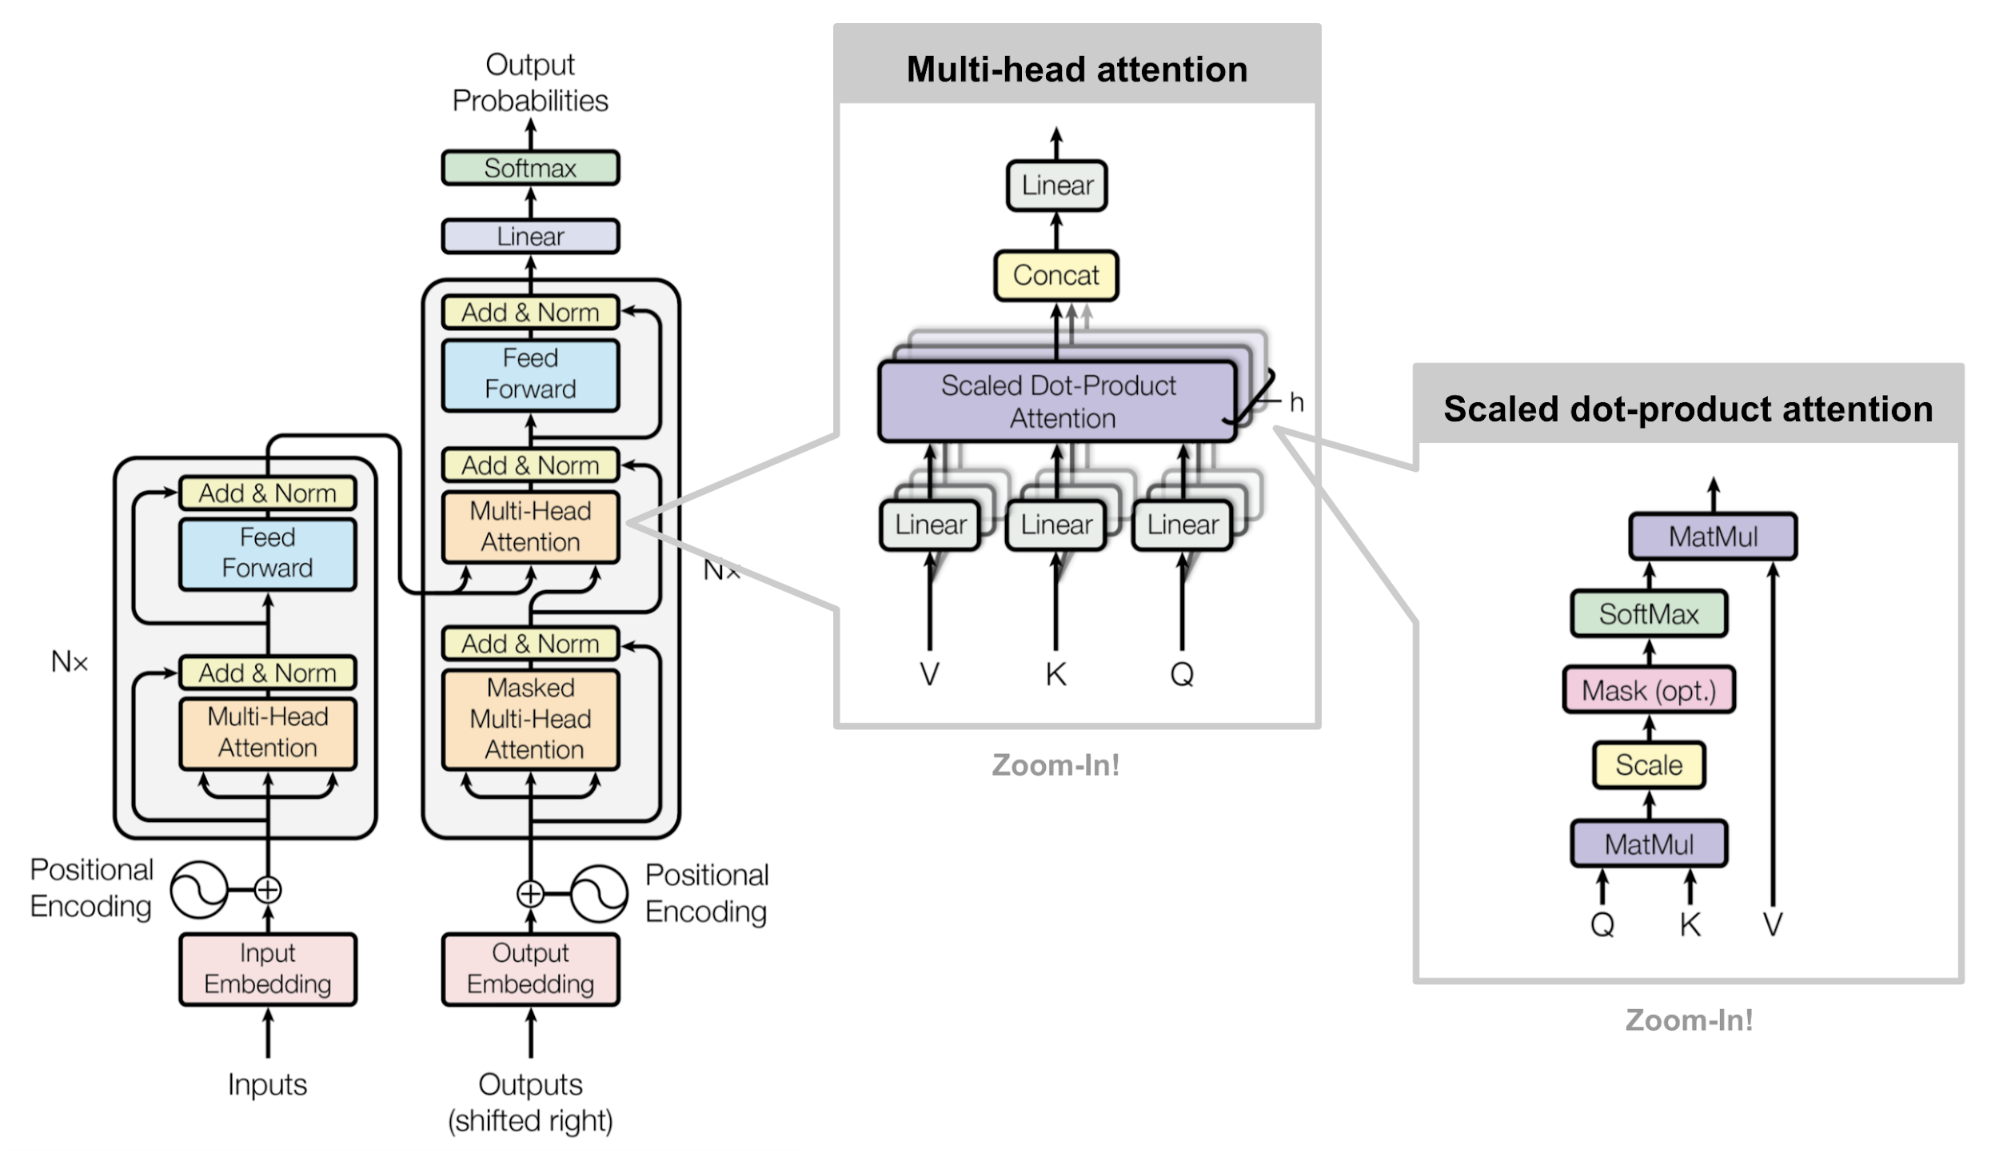
\includegraphics[width=6in]
{transformer/transformer.png}
\caption{Vanilla tranet}
\label{fig-vanilla-transformer}
\end{figure}

Let

$\ell=$ maximum number of words in a sentence segment. $\alp\in [\ell]$, $\ell\sim 100$

$L=$ number of words in vocabulary, $\beta\in[L]$, $L>> \ell$

$d=d_\rvq=d_\rvk=d_\rvv=64$, hidden dimension  per head,
$\delta\in[d]$. 

$n_\rvh=8$, number of heads, $\nu \in[n_\rvh]$

$D=n_\rvh d=8(64)=512$, hidden dimension for all heads,
$\Delta\in [D]$

$\Lambda=6$, number copies,
connected in series,
of boxed bnet, $\lam\in[\Lambda]$

Our tensor notation is discussed in Section 
\ref{sec-numpy-tensors}.
Here is a quick review
of some of the more essential
facts in that section on tensors.
Below will often accompany 
  an equation in tensor
  component notation
  with, in parenthesis, the equivalent matrix equation.
 
 

\begin{itemize}

\item{\bf reshaping}

\beq
T^{\nu, \delta}\rarrow T^{\Delta}
\;\;
\left(
T^{[n_\rvh], [d]} \rarrow T^{[D]}
\right)
\eeq

\beq
T^{\Delta}\rarrow T^{\nu, \delta}
\;\;
\left(
T^{[D]}\rarrow T^{[n_\rvh], [d]}
\right)
\eeq

\item {\bf concatenation}
\beq
T^{[n]}= (T^0, T^1,\ldots, T^{n-1})= 
(T^\nu)_{\nu\in[n]}
\eeq

\item {\bf Hadamard product (element-wise, entry-wise multiplication)}
\beq
T^{[n]}* S^{[n]}= (T^\nu S^\nu)_{\nu\in[n]}
\eeq


\item {\bf Matrix multiplication}

$T^{[n]}= T^{[n], [1]}$ is a column vector.

\beq
(T^{[n]})^T S^{[n]}=\text{scalar}
\eeq

\beq
T^{[a],[b]}S^{[b], [c]}
=\left[\sum_{\beta\in[b]} T^{\alp, \beta}
S^{\beta, \gamma}\right]
_{\alp_\in [a], \gamma \in [c]}
\eeq

Most treatments of tranets, including the
``Attention is all you need" paper,  order the
operations chronologically from
left to right. So if $A$ occurs before $B$,
they write $AB$.
This is contrary 
to what is done in Linear Algebra, where one 
orders the operations chronologically from right to left, and one writes $BA$.
We will adhere to the Linear Algebra
convention, since it is so prevalent
and is the overwhelming precedent.
\end{itemize}



Before we present the bnet
version of Fig.\ref{fig-vanilla-transformer},
we discuss some of the 
definitions needed to
understand and motivate
 Fig.\ref{fig-vanilla-transformer}.
 
 
 \begin{itemize}
 
 \item {\bf Encoder Input $x^{\beta, \alp}$}
 \beq
 x^{\beta, \alp} =\delta(\beta, \beta(\alp))
 \left(
 x^{[L], [\ell]} \text{ has one hot columns.}
 \right)
 \eeq

\item {\bf Embedding (a.k.a. encoding) Matrix $E^{\delta, \beta}$}

\beq
e^{\delta, \alp} = \sum_\beta 
E^{\delta, \beta}
x^{\beta, \alp}
\;\;
\left(
e^{[d],[\ell]}= E^{[d], [L]}x^{[L], [\ell]}
\right)
\eeq

\item{\bf Weight matrices $W_\rvq, W_\rvk, W_\rvv$}

\beq
Q^{\nu,\delta, \alp}=\sum_{\delta'}
W_\rvq^{\nu, \delta, \delta'}e^{\delta', \alp}
\;\;
\left(
Q^{[D], [\ell]}=
W_\rvq^{[D],[d]}E^{[d],[\ell]}
\right)
\eeq


\beq
K^{\nu,\delta, \alp}=
\sum_{\delta'}
W_\rvk^{\nu, \delta, \delta'}
e^{\delta', \alp}
\;\;
\left(
K^{[D], [\ell]}=
W_\rvk^{[D],[d]}E^{[d],[\ell]}
\right)
\eeq

\beq
V^{\nu,\delta, \alp}=
\sum_{\delta'}
W_\rvv^{\nu, \delta, \delta'}
e^{\delta', \alp}
\;\;
\left(
V^{[D], [\ell]}=
W_\rvv^{[D],[d]}E^{[d],[\ell]}
\right)
\eeq

\item {\bf Multi-head Attention}

\beq
B^{
\nu,{\alp'}, \alp}=
\frac{1}{\sqrt{d}}
\sum_\delta K^{\nu,\delta,{\alp'}}
Q^{\nu,\delta,\alp}
\;\;
\left(
B^{[n_h],[\ell],[\ell]}
=\left[
\frac{1}{\sqrt{d}}
(K^{\nu, [d], [\ell]})^T
Q^{\nu, [d], [\ell]}\right]_{\nu\in[n_\rvh]}
\right)
\eeq

\beqa
A^{\nu, 
\delta, \alp}&=&
\sum_{{\alp'}}
V^{\nu, \delta, {\alp'}}
\underbrace{
{\rm softmax}(B^{\nu, [\ell],\alp})(\alp'|\alp, \nu)}_{
P({\alp'}|\alp, \nu)}
\eeqa

\beq
\sum_{{\alp'}\in [\ell]}P({\alp'}| \alp, \nu)=1
\eeq

\beq
A^{\nu, \delta, \alp}
\rarrow
A^{\Delta, \alp}
\left(
A^{[n_\rvh], [d], [\ell]}
\rarrow
A^{[D], [\ell]}\right)
\eeq

Column vector notation:

\beq
B^{\nu, {\alp'}, \alp}=
\frac{1}{\sqrt{d}}
(K^{\nu, [d], {\alp'}})^T Q^{\nu, [d], \alp}
\eeq
Important: Note that the softmax() makes the
${\alp'}$ component a probability,
not the $\alp$ one!

For example, suppose $\nu=1$ (one head), $\ell=2$ (a 2 word segment), 
and $d=3$ (hidden dimension is 3).
The $Q^{[3], [2]}, K^{[3], [2]}, V^{[3], [2]}$ are $3\times 2$ matrices
(i.e., two 3-dim column vectors).
One uses the $Q^{[3], [2]}$ and $K^{[3], [2]}$ to arrive at a 
$2\times 2$ matrix $P(\alp'|\alp)$
of probabilities.
Then one uses that matrix of probabilities to replace

\beq
\left[
V^{[3], 0}, V^{[3], 1} 
\right]
\rarrow
\left[
V^{[3], 0} P(0|0)
+ 
V^{[3], 1}P(1|0)
,
V^{[3], 0} P(0|1)
+ 
V^{[3], 1}P(1|1)
\right]
\eeq

\item{\bf Positional Embedding Matrix
$E_{pos}^{\delta,\beta}$}
 


\beq
E_{pos}^{\delta, \beta}=
\left\{
\begin{array}{ll}
\sin\left(2\pi\frac{\beta}
{(2\pi)10^{4\delta/d}}\right)= \sin(2\pi \frac{\beta}{\lam(\delta)})
& \text{if $\delta$ is even}
\\
\cos\left(2\pi\frac{\beta}{(2\pi)10^{4(\delta-1)/d}}\right)=
\cos(2\pi\frac{\beta}{\lam(\delta)})
& \text{if $\delta$ is odd}
\end{array}
\right.
\eeq
$E_{pos}^{\delta, \beta}$ changes in phase by $\pi/2$  
every time $\delta$ changes by 1. Its wavelength 
$\lam$ is independent
of $\beta$, but increases rapidly with $\delta$, from $\lam(\delta=0)=2\pi*1$ to 
$\lam(\delta=d)= 2\pi* 10^4$.

Total Embedding equals initial embedding plus 
positional embedding:

\beq
E^{\delta, \beta} = E_0^{\delta, \beta} + E_{pos}^{\delta, \beta}
\eeq


The purpose of positional embedding is to take $e^{\beta, \alp}$ to $e^{\delta, \alp}=
\sum_\beta E^{\delta,\beta}_{pos} e^{\beta, \alp}$
where $e^{\delta, \alp}$ changes quickly as $\delta$ (i.e., position) changes.

\item {\bf ReLU}

For a tensor $T$ of arbitrary shape,
\beq
ReLU(T) = (T)_+ = max(0, T)
\eeq
max element-wise.

\item {\bf Feed Forward Neural Net}


\beq
F(e^{\delta, \alp}) = \sum_{\Delta\in[n_{ff}]} W_2^{\delta, \Delta}ReLU\left(\sum_{\delta'\in [d]}
W_1^{\Delta, \delta'}e^{\delta', \alp} + b_1^{\Delta, \alp}\right)  + b_2^{\delta, \alp}
\eeq

$n_{ff}$ is called the {\tt intermediate\_size}
in BERT.

\item {\bf Softmax}

softmax() takes a vector and returns
a vector of probabilities of the same length

\beq
e^{[n]}\rarrow P^{[n]}
\eeq
where

\beq
P^\alp=
\frac{\exp(e^\alp)}
{\sum_{\alp\in[n]} \exp(e^\alp )}
\;\;
\left(P^{[n]}=\frac{\exp(e^{[n]})}
{\norm{\exp(e^{[n]})
}_0}
\right)
\eeq

For example,
\beq
(1,0,0)\rarrow (e,1,1)/norm
\eeq

\beq
(10,0,0)\rarrow (e^{10}, 1, 1)/norm \approx (1,0,0)
\eeq

For any $a\in\RR$,
\beq
(a,a,a)\rarrow \frac{1}{3}(1, 1, 1)
\eeq


\item {\bf Skip Connection (Add \& Normalize)}

A {\bf skip connection} is when you split the
input to a {\bf filter} into two streams, one stream goes through
the filter, the other doesn't. The one that doesn't
is then merged with the output of the filter via a {\bf add \& normalize} node. The reason for making skip connections
is that the signal exiting a filter is usually full of
jumps and kinks. By merging that filter output
with some  of the filter input, one smooths out the filter output
to some degree. This makes back-propagation differentiation
better behaved.

The filter might be a Multi-Head Attention or a Feed Forward NN.

Add \& Normalize just means $(A + B)/norm$ where $A$ and $B$
are the two input signals and ``norm" is some norm of $A+B$ (for
instance, $\norm{A+B}_2$).

Normalization keeps the signal from growing too big and saturating the signal that will enter components upstream.
Normalization can also involve subtracting the mean $\av{X}$ of the signal $X$  so as to get a signal $X-\av{X}$  that has zero mean.

%\item {\bf Plates}
%
%Fig.\ref{fig-vanilla-transformer}
%uses plates (a.k.a. stacks). These are explained in Chapter \ref{ch-plates}.


\item {\bf Redundancy}

For better results, the Encoder
and Decoder both contain $\Lam$ 
copies, connected in series, of the boxed bnet.

\item{\bf Right Shifted Outputs}

``Outputs (Shifted Right)" in Fig.\ref{fig-vanilla-transformer}
refers to what is called
{\bf forced teaching}
in the RNN (recurrent neural net) 
literature.
We explain forced teaching
in Fig.\ref{fig-transformer-full-3-words-train-test}.


\begin{figure}[!h]
\centering
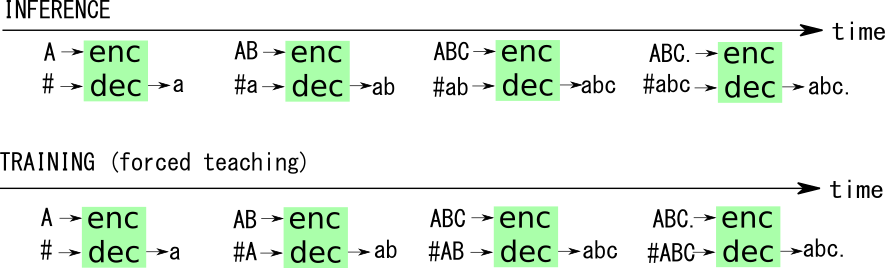
\includegraphics[width=6in]
{transformer/transformer-train-test.png}
\caption{Training and Inference for vanilla transformer.
``enc" and ``dec" denote
the encoder and decoder, respectively.
A hash character represents the SOS (start of sentence) token,
and a period represents the EOS (end of sentence) token. Capital letters represent ground
truth tokens, and lower case ones represent 
predictions.}
\label{fig-transformer-full-3-words-train-test}
\end{figure}

\item {\bf Masked Attention}

\beq
P(\alp'|\alp, \nu) = 0 \;\;\;
\text{ if $\alp'<\alp$}
\eeq
$\alp$, and $\alp'$ are
sentence positions and $\alp'$ is in the future (downstream)
compared to $\alp$.
So as to
not violate causality,
this condition enforces the constraint that no attention is paid to sentence positions in the future of $\alp$.


%\item {\bf plates}
%
%Fig.\ref{fig-vanilla-transformer}
%uses plates (a.k.a. stacks). These are explained in Chapter \ref{ch-plates}.


\end{itemize}

\subsection{Single Head Attention}

Fig.\ref{fig-texnn-for-scaled-dot-prod-att}
gives a
bnet representation of
the ``Single Head Attention"
portion of Fig.\ref{fig-vanilla-transformer}.
The structural equations for that bnet,
printed in blue,
are as follows.
 

\begin{figure}[!h]\centering
\begin{minipage}{.5\linewidth}
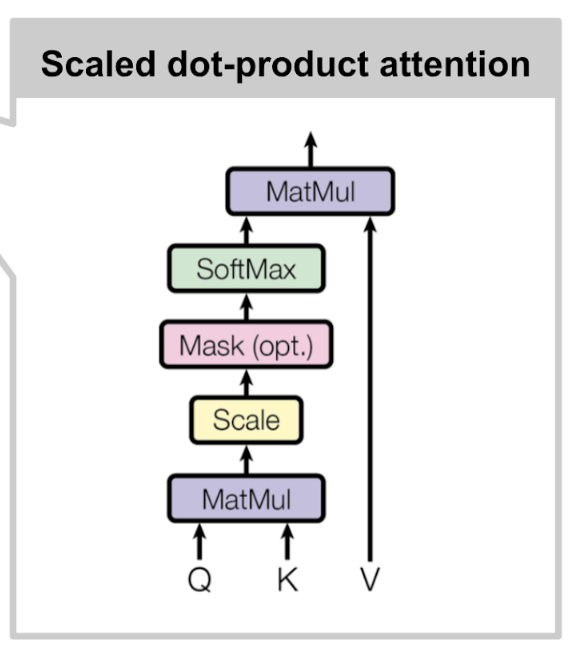
\includegraphics[width=2in]{transformer/scaled-dot-prod-att.jpg}
\end{minipage}%blank lines between minispaces breaks this
\begin{minipage}{.5\linewidth}
$$\xymatrix{
*+[F*:Orchid]{\underline{A}^{[d], [\ell]}}&&&
\\
&&*+[F*:SpringGreen]{\underline{P}^{[\ell], [\ell]}}\ar[ull]&
\\
&&*+[F*:Lavender]{\underline{M}^{[\ell], [\ell]}}\ar[u]&
\\
&&*+[F*:yellow]{\underline{S}^{[\ell],[\ell]}}\ar[u]&
\\
&&*+[F*:Orchid]{\underline{B}^{[\ell], [\ell]}}\ar[u]&
\\
*+[F*:Orchid]{\underline{V}^{[d],[\ell]}}\ar[uuuuu]&*+[F*:Orchid]{\underline{K}^{[d],[\ell]}}\ar[ur]&&*+[F*:Orchid]{\underline{Q}^{[d],[\ell]}}\ar[ul]
}$$
\end{minipage}
\caption{Single Head Attention. (Scaled Dot Product)}
\label{fig-texnn-for-scaled-dot-prod-att}
\end{figure}

\begin{subequations}

\begin{equation}\color{blue}
A^{[d], [\ell]} = V^{[d],[\ell]} P^{[\ell], [\ell]}\;\;\text{$\left(\text{Note that }\sum_{\alp\in[\ell]} P^{\alp, [\ell]}=1\right)$}
\label{eq-P-fun-scaled-dot-prod-att}
\end{equation}

\begin{equation}\color{blue}
B^{[\ell], [\ell]} = (K^{[d],[\ell]})^T Q^{[d],[\ell]}
\label{eq-B-fun-scaled-dot-prod-att}
\end{equation}

\begin{equation}\color{blue}
K^{[d],[\ell]} = \;\;\text{prior}
\label{eq-K-fun-scaled-dot-prod-att}
\end{equation}

\begin{equation}\color{blue}
M^{[\ell], [\ell]} = \text{mask}(S^{[\ell],[\ell]})
\label{eq-R-fun-scaled-dot-prod-att}
\end{equation}

\begin{equation}\color{blue}
P^{[\ell], [\ell]} = \text{softmax}(M^{[\ell], [\ell]})\;\;\text{$\left(\text{Note that }\sum_{\alp\in[\ell]} P^{\alp, [\ell]}=1\right)$}
\label{eq-G-fun-scaled-dot-prod-att}
\end{equation}

\begin{equation}\color{blue}
Q^{[d],[\ell]} = \;\;\text{prior}
\label{eq-Q-fun-scaled-dot-prod-att}
\end{equation}

\begin{equation}\color{blue}
S^{[\ell],[\ell]} = \frac{B^{[\ell], [\ell]}}{\sqrt{d}}
\label{eq-Y-fun-scaled-dot-prod-att}
\end{equation}

\begin{equation}\color{blue}
V^{[d],[\ell]} = \;\;\text{prior}
\label{eq-V-fun-scaled-dot-prod-att}
\end{equation}

\end{subequations}

\subsection{Multi-Head Attention}

Fig.\ref{fig-texnn-for-multi-head-att}
gives a
bnet representation of
the ``Multi-Head Attention"
portion of Fig.\ref{fig-vanilla-transformer}.
The structural equations for that bnet,
printed in blue, are as follows.

\begin{figure}[!h]\centering
\begin{minipage}{.3\linewidth}
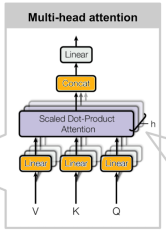
\includegraphics[width=1.7in]{transformer/multi-head-att.png}
\end{minipage}%blank lines between minispaces breaks this
\begin{minipage}{.7\linewidth}
$$\xymatrix@C=1.3pc{
&&*+[F*:Orchid]{\underline{Q_0}^{[d],[\ell]}}\ar[dddr]&&&
\\
&*+[F*:Dandelion]{\underline{Q}^{[D], [\ell]}}\ar[ur]\ar[dr]&&&&
\\
&&*+[F*:Orchid]{\underline{Q_1}^{[d],[\ell]}}\ar[dddr]&&&
\\
&&*+[F*:Orchid]{\underline{K_0}^{[d],[\ell]}}\ar[r]&*+[F*:Orchid]{\underline{A_0}^{[d],[\ell]}}\ar[dr]&&
\\
*+[F*:SpringGreen]{\underline{e}^{[d], [\ell]}}\ar[r]^{W_\rvk}\ar[uuur]^{W_\rvq}\ar[dddr]^{W_\rvv}&*+[F*:Dandelion]{\underline{K}^{[D], [\ell]}}\ar[ur]\ar[dr]&&&*+[F*:Dandelion]{\underline{A}^{[D],[\ell]}}\ar[r]^{W_\rva}&*+[F*:SpringGreen]{\underline{O}^{[d],[\ell]}}
\\
&&*+[F*:Orchid]{\underline{K_1}^{[d],[\ell]}}\ar[r]&*+[F*:Orchid]{\underline{A_1}^{[d],[\ell]}}\ar[ur]&&
\\
&&*+[F*:Orchid]{\underline{V_0}^{[d],[\ell]}}\ar[uuur]&&&
\\
&*+[F*:Dandelion]{\underline{V}^{[D], [\ell]}}\ar[ur]\ar[dr]&&&&
\\
&&*+[F*:Orchid]{\underline{V_1}^{[d],[\ell]}}\ar[uuur]&&&
}$$
\end{minipage}
\caption{Multi-head Attention with 2 heads. Note that the orange nodes all have the same tensor shape.}
\label{fig-texnn-for-multi-head-att}
\end{figure}

\begin{subequations}

\begin{equation}\color{blue}
A^{[D],[\ell]} = [A_0^{[d],[\ell]}|A_1^{[d],[\ell]}]
\label{eq-C-fun-multi-head-att}
\end{equation}

\begin{equation}\color{blue}
A_0^{[d],[\ell]} = \text{Attention}(V_0^{[d],[\ell]},K_0^{[d],[\ell]},Q_0^{[d],[\ell]})
\label{eq-X-fun-multi-head-att}
\end{equation}

\begin{equation}\color{blue}
A_1^{[d],[\ell]} = \text{Attention}(V_1^{[d],[\ell]},K_1^{[d],[\ell]},Q_1^{[d],[\ell]})
\label{eq-Y-fun-multi-head-att}
\end{equation}

\begin{equation}\color{blue}
K^{[D], [\ell]} = W_\rvk^{[D],[d]}e^{[d], [\ell]}
\label{eq-K-fun-multi-head-att}
\end{equation}

\begin{equation}\color{blue}
K_0^{[d],[\ell]} = \text{linear}(K^{[D], [\ell]})\;\;\text{(split, then project a component)}
\label{eq-4-fun-multi-head-att}
\end{equation}

\begin{equation}\color{blue}
K_1^{[d],[\ell]} = \text{linear}(K^{[D], [\ell]})\;\;\text{(split, then project a component)}
\label{eq-5-fun-multi-head-att}
\end{equation}

\begin{equation}\color{blue}
O^{[d],[\ell]} = W_\rva^{[d],[D]}A^{[D],[\ell]}
\label{eq-F-fun-multi-head-att}
\end{equation}

\begin{equation}\color{blue}
Q^{[D], [\ell]} = W_\rvq^{[D],[d]}e^{[d], [\ell]}
\label{eq-Q-fun-multi-head-att}
\end{equation}

\begin{equation}\color{blue}
Q_0^{[d],[\ell]} = \text{linear}(Q^{[D], [\ell]})\;\;\text{(split, then project a component)}
\label{eq-1-fun-multi-head-att}
\end{equation}

\begin{equation}\color{blue}
Q_1^{[d],[\ell]} = \text{linear}(Q^{[D], [\ell]})\;\;\text{(split, then project a component)}
\label{eq-2-fun-multi-head-att}
\end{equation}

\begin{equation}\color{blue}
V^{[D], [\ell]} = W_\rvv^{[D],[d]}e^{[d], [\ell]}
\label{eq-V-fun-multi-head-att}
\end{equation}

\begin{equation}\color{blue}
V_0^{[d],[\ell]} = \text{linear}(V^{[D], [\ell]})\;\;\text{(split, then project a component)}
\label{eq-7-fun-multi-head-att}
\end{equation}

\begin{equation}\color{blue}
V_1^{[d],[\ell]} = \text{linear}(V^{[D], [\ell]})\;\;\text{(split, then project a component)}
\label{eq-8-fun-multi-head-att}
\end{equation}

\begin{equation}\color{blue}
e^{[d], [\ell]} = \;\;\text{prior}
\label{eq-e-fun-multi-head-att}
\end{equation}

\end{subequations}


\subsection{Encoder}

Fig.\ref{fig-texnn-for-encoder}
gives a
bnet representation of
the ``Encoder"
portion of Fig.\ref{fig-vanilla-transformer}.
The structural equations for that bnet,
printed in blue, are as follows.


\begin{figure}[!h]\centering
\begin{minipage}{.4\linewidth}
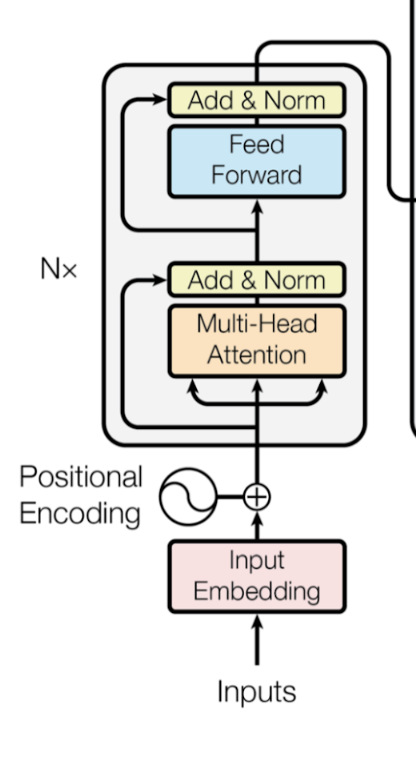
\includegraphics[width=2in]{transformer/encoder.jpg}
\end{minipage}%blank lines between minispaces breaks this
\begin{minipage}{.6\linewidth}
$$\xymatrix@R=3.5pc@C=0.1pc{
*+[F*:yellow]{\underline{n}^{[d], [\ell]}}&&&
\\
&*+[F*:SkyBlue]{\underline{F}^{[d], [\ell]}}\ar[ul]&&
\\
*+[F*:yellow]{\underline{N}^{[d], [\ell]}}\ar[ur]\ar[uu]&&&
\\
&&*+[F*:Dandelion]{\underline{A}^{[D], [\ell]}}\ar[ull]_{W_\rva}&
\\
&*+[F*:Dandelion]{\underline{Q}^{[D], [\ell]}}\ar[ur]&*+[F*:Dandelion]{\underline{K}^{[D], [\ell]}}\ar[u]&*+[F*:Dandelion]{\underline{V}^{[D], [\ell]}}\ar[ul]
\\
*+[F*:gray]{\underline{e}^{[d], [\ell]}}\ar[urr]^{W_\rvk}\ar[uuu]\ar[ur]^{W_\rvq}\ar[urrr]_{W_\rvv}&&&
\\
*+[F*:Lavender]{\underline{x}^{[L],[\ell]}}\ar[u]&&&
\save
\POS"1,1"."5,1"."1,4"."5,4"!C*+<6.0em>\frm{-,}
\restore
}$$
\end{minipage}
\caption{Encoder of Vanilla Transformer Net. $\Lam$ copies of the boxed part are connected in series.}
\label{fig-texnn-for-encoder}
\end{figure}

\begin{subequations}

\begin{equation}\color{blue}
A^{[D], [\ell]} = \text{Attention}(Q^{[D], [\ell]},K^{[D], [\ell]},V^{[D], [\ell]})
\label{eq-O-fun-encoder}
\end{equation}

\begin{equation}\color{blue}
F^{[d], [\ell]} = \text{feed\_forward\_nn}(N^{[d], [\ell]})
\label{eq-F-fun-encoder}
\end{equation}

\begin{equation}\color{blue}
K^{[D], [\ell]} = W_\rvk^{[D], [d]}e^{[d], [\ell]}
\label{eq-K-fun-encoder}
\end{equation}

\begin{equation}\color{blue}
N^{[d], [\ell]} = \text{normalize}(e^{[d], [\ell]} + W_\rva^{[d],[D]}A^{[D], [\ell]})
\label{eq-N-fun-encoder}
\end{equation}

\begin{equation}\color{blue}
Q^{[D], [\ell]} = W_\rvq^{[D], [d]}e^{[d], [\ell]}
\label{eq-Q-fun-encoder}
\end{equation}

\begin{equation}\color{blue}
V^{[D], [\ell]} = W_\rvv^{[D], [d]}e^{[d], [\ell]}
\label{eq-V-fun-encoder}
\end{equation}

\begin{equation}\color{blue}
e^{[d], [\ell]} = E^{[d], [L]}x^{[L],[\ell]}
\label{eq-p-fun-encoder}
\end{equation}

\begin{equation}\color{blue}
n^{[d], [\ell]} = \text{normalize}(N^{[d], [\ell]} + F^{[d], [\ell]})
\label{eq-n-fun-encoder}
\end{equation}

\begin{equation}\color{blue}
x^{[L],[\ell]} = \;\;\text{prior}
\label{eq-R-fun-encoder}
\end{equation}

\end{subequations}



\subsection{Decoder}

Fig.\ref{fig-texnn-for-decoder}
gives a
bnet representation of
the ``Decoder"
portion of Fig.\ref{fig-vanilla-transformer}.
The structural equations for that bnet,
printed in blue, are as follows.

\begin{figure}[h!]\centering
\begin{minipage}{.4\linewidth}
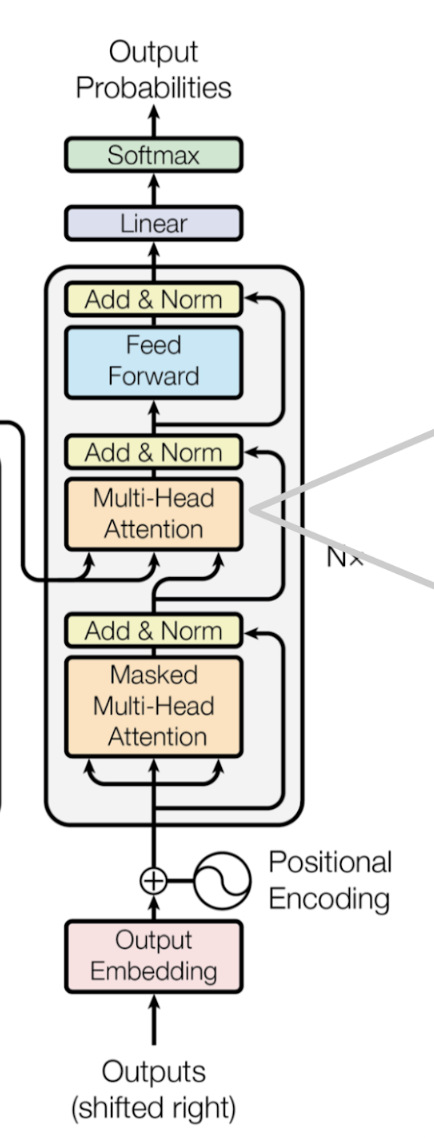
\includegraphics[width=2in]{transformer/decoder.jpg}
\end{minipage}%blank lines between minispaces breaks this
\begin{minipage}{.6\linewidth}
$$\xymatrix@R=3pc@C=0.2pc{
&&&*+[F*:SpringGreen]{\underline{P}^{[L],[\ell]}}
\\
&&&*+[F*:Orchid]{\underline{I}^{[L],[\ell]}}\ar[u]
\\
&&&*+[F*:yellow]{\underline{Y}^{[d], [\ell]}}\ar[u]
\\
&&*+[F*:SkyBlue]{\underline{F}^{[d], [\ell]}}\ar[ur]&
\\
&*+[F*:Dandelion]{\underline{a}^{[D],[\ell]}}\ar[rr]^{U_\rva}&&*+[F*:yellow]{\underline{j}^{[d], [\ell]}}\ar[ul]\ar[uu]
\\
*+[F*:Dandelion]{\underline{v}^{[D], [\ell]}}\ar[ur]&*+[F*:Dandelion]{\underline{k}^{[D], [\ell]}}\ar[u]&*+[F*:Dandelion]{\underline{q}^{[D], [\ell]}}\ar[ul]&
\\
*+[F*:yellow]{\underline{n}^{[d], [\ell]}}\ar[ur]_{U_\rvk}\ar[u]^{U_\rvv}&&&*+[F*:yellow]{\underline{J}^{[d], [\ell]}}\ar[uu]\ar[ul]^{U_\rvq}
\\
&*+[F*:Dandelion]{\underline{A}^{[D],[\ell]}}\ar[urr]^{W_\rva}&&
\\
*+[F*:Dandelion]{\underline{Q}^{[D], [\ell]}}\ar[ur]&*+[F*:Dandelion]{\underline{K}^{[D], [\ell]}}\ar[u]&*+[F*:Dandelion]{\underline{V}^{[D], [\ell]}}\ar[ul]&
\\
&&&*+[F*:gray]{\underline{e}^{[d],[\ell]}}\ar[uuu]\ar[ull]_{W_\rvk}\ar[ulll]^{W_\rvq}\ar[ul]_{W_\rvv}
\\
&&&*+[F*:Lavender]{\underline{x}^{[L],[\ell]}}\ar[u]
\save
\POS"3,1"."9,1"."3,4"."9,4"!C*+<6.0em>\frm{-,}
\restore
}$$
\end{minipage}
\caption{Decoder of Vanilla Transformer Net. $\Lam$ copies of the boxed part are connected in series.}
\label{fig-texnn-for-decoder}
\end{figure}

\begin{subequations}

\begin{equation}\color{blue}
A^{[D],[\ell]} = \text{Attention}(Q^{[D], [\ell]},K^{[D], [\ell]},V^{[D], [\ell]})
\label{eq-o-fun-decoder}
\end{equation}

\begin{equation}\color{blue}
F^{[d], [\ell]} = \text{feed\_forward\_nn}(j^{[d], [\ell]})
\label{eq-B-fun-decoder}
\end{equation}

\begin{equation}\color{blue}
I^{[L],[\ell]} = W^{[L], [d]}Y^{[d], [\ell]}
\label{eq-I-fun-decoder}
\end{equation}

\begin{equation}\color{blue}
J^{[d], [\ell]} = \text{normalize}(W_\rva^{[d], [D]}A^{[D],[\ell]} + e^{[d],[\ell]})
\label{eq-a-fun-decoder}
\end{equation}

\begin{equation}\color{blue}
K^{[D], [\ell]} = W_\rvk^{[D],[d]}e^{[d],[\ell]}
\label{eq-K-fun-decoder}
\end{equation}

\begin{equation}\color{blue}
P^{[L],[\ell]} = \text{softmax}(I^{[L],[\ell]})\;\;\text{$(\sum_{\alp\in[\ell]}P^{[L], \alp}=1)$}
\label{eq-G-fun-decoder}
\end{equation}

\begin{equation}\color{blue}
Q^{[D], [\ell]} = W_\rvq^{[D],[d]}e^{[d],[\ell]}
\label{eq-Q-fun-decoder}
\end{equation}

\begin{equation}\color{blue}
V^{[D], [\ell]} = W_\rvv^{[D],[d]}e^{[d],[\ell]}
\label{eq-V-fun-decoder}
\end{equation}

\begin{equation}\color{blue}
Y^{[d], [\ell]} = \text{normalize}(F^{[d], [\ell]} + J^{[d], [\ell]})
\label{eq-Y-fun-decoder}
\end{equation}

\begin{equation}\color{blue}
a^{[D],[\ell]} = \text{Attention}(v^{[D], [\ell]},k^{[D], [\ell]},q^{[D], [\ell]})
\label{eq-O-fun-decoder}
\end{equation}

\begin{equation}\color{blue}
e^{[d],[\ell]} = E^{[d],[L]}x^{[L],[\ell]}
\label{eq-p-fun-decoder}
\end{equation}

\begin{equation}\color{blue}
j^{[d], [\ell]} = \text{normalize}(U_\rva^{[d],[D]}a^{[D],[\ell]} + J^{[d], [\ell]})
\label{eq-j-fun-decoder}
\end{equation}

\begin{equation}\color{blue}
k^{[D], [\ell]} = U_\rvk^{[D],[d]}n^{[d], [\ell]}
\label{eq-k-fun-decoder}
\end{equation}

\begin{equation}\color{blue}
n^{[d], [\ell]} = \;\;\text{Prior coming from Encoder.}
\label{eq-n-fun-decoder}
\end{equation}

\begin{equation}\color{blue}
q^{[D], [\ell]} = U_\rvq^{[D],[d]}J^{[d], [\ell]}
\label{eq-q-fun-decoder}
\end{equation}

\begin{equation}\color{blue}
v^{[D], [\ell]} = U_\rvv^{[D], [d]}n^{[d], [\ell]}
\label{eq-v-fun-decoder}
\end{equation}

\begin{equation}\color{blue}
x^{[L],[\ell]} = \;\;\text{prior, right shifted output}
\label{eq-R-fun-decoder}
\end{equation}

\end{subequations}

\section{BERT}

BERT is a realization of the Encoder part of the Vanilla tranet.

% Please add the following required packages to your document preamble:
% \usepackage[table,xcdraw]{xcolor}
% Beamer presentation requires \usepackage{colortbl} instead of \usepackage[table,xcdraw]{xcolor}
\begin{table}[!h]
\centering
\begin{tabular}{|l|l|l|}
\hline
 & \cellcolor[HTML]{FFFFC7}BERT base & \cellcolor[HTML]{FFFFC7}BERT large \\ 
 \hline
\cellcolor[HTML]{FFFFC7}$\ell$ & 512? & 512? \\ \hline
\cellcolor[HTML]{FFFFC7}$L$, {\tt vocab\_size} & 30,522 & 30,522 \\ \hline
\cellcolor[HTML]{FFFFC7}$d$, {\tt hidden\_size} & 768 & 768 \\ \hline
\cellcolor[HTML]{FFFFC7}$n_\rvh$, {\tt num\_attention\_heads} & 12 & 12 \\ \hline
\cellcolor[HTML]{FFFFC7}$\Lambda$, {\tt num\_hidden\_layers} & 12 & 24 \\ \hline
\cellcolor[HTML]{FFFFC7}$n_{ff}$, {\tt intermediate\_size} & 3,072 & 3,072 \\ \hline
\end{tabular}
\caption{Some hyperparameters for BERT base and BERT large}
\label{tab-bert}
\end{table}